\section{Method}\label{sec:method}

We describe SoundCode along four axes. Section~\ref{sec:arch} gives the
system architecture and identifies the four components that change
relative to a synchronous baseline. Section~\ref{sec:algo} presents
the producer-consumer decoding loop in pseudocode. Sections
\ref{sec:when-async}--\ref{sec:where-rollback} answer the three design
questions inherited from
ROCODE \citep{jiang2024rocode} and reframed by the async setting:
\emph{when} to run the verifier asynchronously, \emph{when} to roll
back, and \emph{where} to roll back to. Section~\ref{sec:impl}
summarizes the implementation.

\subsection{System architecture}\label{sec:arch}

\begin{figure}[t]
  \centering
  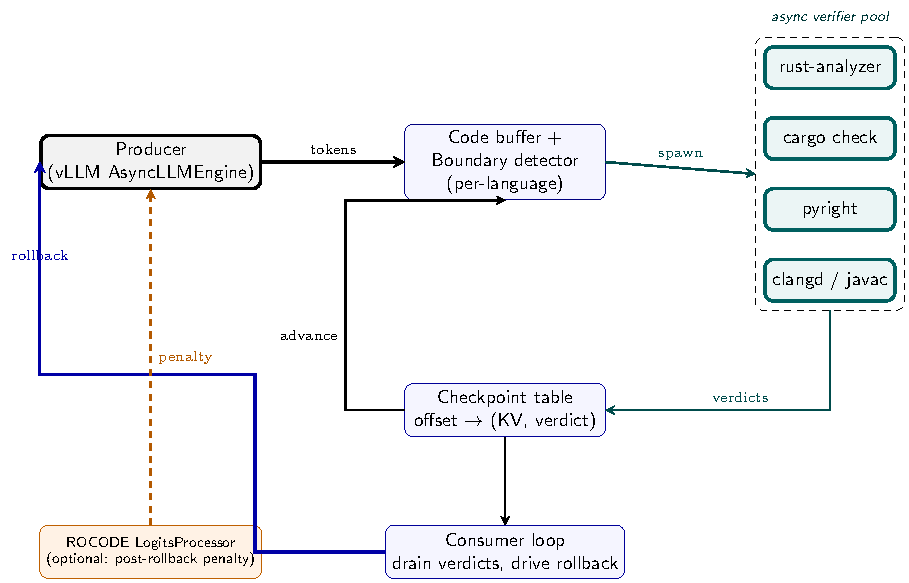
\includegraphics[width=\linewidth]{figures/architecture.pdf}
  \caption{SoundCode's producer-consumer architecture. The producer
    LM streams tokens; a structural boundary detector identifies
    depth-zero \code{;} and \code{\}} in the function body; at each
    boundary an async verifier task is spawned on a snapshot of the
    current buffer; a consumer drains finished verifier tasks in
    FIFO order; on the first blocking diagnostic, pending tasks are
    cancelled and the buffer is rolled back to the most recent
    boundary checkpoint.}
  \label{fig:arch}
\end{figure}

Four components change relative to the synchronous baseline:
\begin{enumerate}[itemsep=2pt,topsep=2pt]
\item A \textbf{structural boundary detector} that, given the running
  token buffer, identifies the points at which a verifier call should
  be triggered. We use depth-zero \code{;} and \code{\}} for the
  C-family languages (Rust, C++, Java); newline at indent zero for
  Python. The detector is language-specific but stateless across
  generations.
\item An \textbf{async verifier task} that, given a snapshot of the
  buffer at a boundary, runs the compiler / LSP server and returns a
  diagnostic classified as \textsc{Blocking}, \textsc{Incomplete}, or
  \textsc{NonBlocking}. Tasks are spawned at boundary time and never
  share state; \code{cargo check} reuses the workspace's incremental
  cache across calls.
\item A \textbf{verifier queue} of in-flight tasks, ordered by spawn
  time. The consumer polls this queue on a tight schedule (every
  $K$ tokens; we use $K\!=\!1$) and removes completed tasks left to
  right. (The reference implementation degenerates the queue to a
  single in-flight check: a boundary spawns a task only when none
  is pending, which coalesces closely-spaced boundaries into the
  next check.)
\item A \textbf{rollback driver} that, on the first
  \textsc{Blocking} diagnostic, cancels pending tasks, truncates the
  buffer to the most recent boundary checkpoint (backing off to
  earlier checkpoints on successive retries), and
  re-prompts the LM from that prefix.
\end{enumerate}

The producer task is the LM, unmodified except for an \code{abort()}
hook that lets the rollback driver interrupt an in-progress
generation. We run inference with vLLM \citep{vllm2023}'s
\code{AsyncLLMEngine}, which natively supports per-request abort and
KV-cache reuse for the surviving prefix; the rollback amounts to
discarding the abandoned suffix and resubmitting the truncated
buffer as a fresh \code{generate()} call.

\begin{figure}[t]
  \centering
  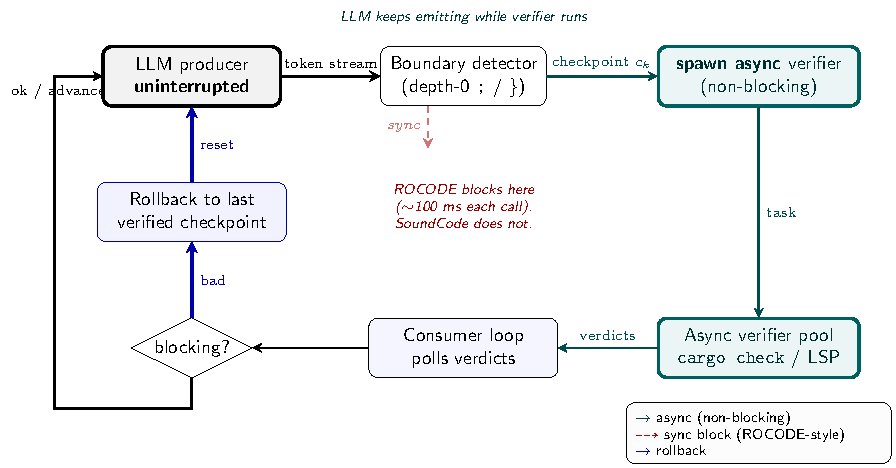
\includegraphics[width=0.85\linewidth]{figures/soundcode_workflow.pdf}
  \caption{SoundCode workflow. The LM (top, black) streams tokens.
    At each depth-zero \code{;}/\code{\}} boundary, an async
    verifier task (teal, dashed) is spawned on a snapshot of the
    buffer. The decoder \emph{does not block} on the verifier ---
    where ROCODE \citep{jiang2024rocode} would (ghost red arrow,
    omitted in SoundCode), control returns immediately to the
    producer. The consumer (blue) drains finished verifier tasks
    in FIFO order. On the first \textsc{Blocking} diagnostic,
    pending tasks are cancelled and the buffer is rolled back to
    the most recent boundary checkpoint.}
  \label{fig:soundcode-workflow}
\end{figure}

At end of stream, the consumer awaits any in-flight verifier tasks
before returning, and a trailing blocking verdict still triggers
rollback and regeneration. Note that checkpoints are recorded
eagerly at boundary time (\S\ref{sec:where-rollback}), so
mid-stream checkpoints are \emph{candidate} rollback targets rather
than verifier-cleared positions; final well-formedness is
established by the end-of-stream drain plus the post-hoc
compile-and-test evaluation.

\subsection{Algorithm}\label{sec:algo}

Algorithm~\ref{alg:soundcode} states the decoding loop. We follow
the ROCODE Algorithm-2 structure \citep{jiang2024rocode}; the
critical difference is that lines~\ref{algline:spawn} and
\ref{algline:consume} run as separate coroutines rather than as
sequential statements, and the rollback test at
line~\ref{algline:rb-test} acts on already-completed verifier tasks
rather than blocking on the just-scheduled one.

\begin{algorithm}[t]
\caption{SoundCode asynchronous compiler-supervised decoding.}\label{alg:soundcode}
\KwIn{prompt $x$; LM $\mathcal{M}$; verifier $\mathcal{V}$; boundary
  detector $\mathcal{B}$; rollback policy $\pi$}
\KwOut{verified completion $y$}
\textbf{queue} $Q \gets \emptyset$\;
\textbf{checkpoints} $C \gets \{0\}$ \tcp*{boundary token indices (eager)}
buffer $y \gets$ empty\;
\textbf{spawn} producer:
  \While{not EOS \textbf{and} not aborted}{
    $t \gets \mathcal{M}.\textsc{next}(x, y)$\;
    $y \gets y \cdot t$\;
    \If(\tcp*[f]{e.g.\ depth-0 \code{;} or \code{\}}}\label{algline:spawn}){
        $\mathcal{B}(y)$}{
      $C \gets C \cup \{|y|\}$ \tcp*{checkpoint recorded at boundary}
      $Q.\textsc{push}(\textsc{spawn-async}~\mathcal{V}(y),
        \text{idx}=|y|)$\;
    }
  }
\textbf{spawn} consumer:
  \While{producer running \textbf{or} $Q \neq \emptyset$}{
    \While(\label{algline:consume}){$Q$ has a completed head $h$}{
      $d \gets h.\textsc{result}$\;
      \uIf{$d$ is \textsc{Blocking}}{\label{algline:rb-test}
        cancel pending tasks; $Q \gets \emptyset$\;
        $\mathcal{M}.\textsc{abort}$\;
        $r \gets \pi(y, d, C)$ \tcp*{rollback target (\S\ref{sec:where-rollback})}
        $y \gets y[:r]$;\quad
        $C \gets \{c \in C : c < r\}$ \tcp*{pop used checkpoint}
        \textbf{restart} producer with prompt $x \cdot y$\;
      }
      \uElseIf{$d$ is \textsc{NonBlocking}}{
        \tcp{no state change --- checkpoint was recorded at boundary}
      }
    }
    \textsc{yield} \tcp*{cooperative; back to producer}
  }
\KwRet{$y$}
\end{algorithm}

The algorithm is parameterized by the rollback policy $\pi$, which
maps a (buffer, diagnostic, checkpoint set) triple to a token
offset. The concrete instantiations are defined in
Section~\ref{sec:where-rollback}: \textsc{NaiveLast} (return
$\max C$), \textsc{RecBackoff} (\textsc{NaiveLast}, but back off one
additional checkpoint when the same error recurs at the same line),
\textsc{ROCODEEntropy} (try error-line offset, fall back
to max-entropy on recurrence), and \textsc{NaiveLast+Penalty} (return
$\max C$ and add ROCODE's
$\lambda^{t-r}$ token penalty to the retry).

\subsection{When to async: a verifier-cost spectrum}\label{sec:when-async}

The motivating constraint is that asynchronous verification only
pays off when the verifier is slow enough that the per-token
generation budget is dominated by verifier idle time. Table
\ref{tab:verifier-cost} sorts the verifiers used by the
closest-neighbour systems along this axis.

\begin{table}[t]
\centering
\caption{Verifier cost spectrum. Times are typical per-call on a
  single CPU core (compiler/LSP verifiers) or a modern GPU (the
  learned-classifier row). Per-token LM cost is
  $\sim$$10$--$30\,\mathrm{ms}$
  for a 7B-class model. The async / sync prediction is whether
  per-call verifier cost exceeds per-token LM cost.}
\label{tab:verifier-cost}
\footnotesize
\begin{tabular}{lllc}
\toprule
Verifier & Used by & Typical per-call cost & Async pays? \\
\midrule
Python \code{compile()} & ROCODE \citep{jiang2024rocode}
  & ${\sim}0.1\,\mathrm{ms}$ & no \\
$g{+}{+}\;\code{-fsyntax-only}$ & ROCODE \citep{jiang2024rocode}
  & ${\sim}3\,\mathrm{ms}$ & marginal \\
SemGuard 1.3B classifier & SemGuard \citep{wang2025semguard}
  & ${\sim}10\,\mathrm{ms}$ & marginal \\
LSP completions (Java JDT) & MGD \citep{agrawal2023monitor}
  & ${\sim}20$--$80\,\mathrm{ms}$ & yes \\
\code{cargo check} (incremental) & SoundCode (this work)
  & ${\sim}35$--$500\,\mathrm{ms}$ & yes \\
\code{javac} (warm JVM) & SoundCode (follow-up) & ${\sim}180\,\mathrm{ms}$ & yes \\
LSP completions (rust-analyzer) & SoundCode (follow-up, \S\ref{sec:extended})
  & ${\sim}50$--$300\,\mathrm{ms}$ & yes \\
Whole-crate borrow / trait analysis & --- (unevaluated)
  & ${\sim}500\,\mathrm{ms}$--several\,s & strongly yes \\
\bottomrule
\end{tabular}
\end{table}

\paragraph{Rule of thumb.}
If a single verifier call costs less than a single LM token's wall
time, synchronous verification is the right design --- the
synchronization overhead of spawning, polling, and awaiting will
exceed the saved blocking time, and the simpler architecture is
preferred. ROCODE's choice of synchronous integration is correct
in the millisecond-verifier regime it measured (Python's
\code{compile()}; warm single-file $g{+}{+}$ parses); SoundCode's
contribution is to show what happens when this inequality flips.
In our decoding loop, per-invocation $g{+}{+}$ cost amortizes to
$\sim$$0.55$\,s (\S\ref{sec:headline-contrast}), which already
flips the inequality on C++; on Rust, \code{cargo check} amortizes
to $\sim$$0.20$\,s --- $\sim$$7$--$20\times$ a per-token decoding
step; the trade-off is no longer marginal. Section~\ref{sec:results} measures
these per-language costs empirically and confirms that async
delivers wall-time wins at the $\sim$$150\,\mathrm{ms}$-or-more
per-call verifier cost regime ($g{+}{+}\;\code{-fsyntax-only}$
amortized at $\sim$$0.55$\,s and \code{cargo check} amortized at
$\sim$$0.20$\,s in our setup --- both above the per-token decode
budget of $\sim$$10$--$30\,\mathrm{ms}$).

\subsection{When to roll back}\label{sec:when-rollback}

The decision to roll back depends on two predicates:
\begin{enumerate}[itemsep=2pt,topsep=2pt]
\item the verifier diagnostic is classified as \textsc{Blocking}
  (we define the classifier below);
\item the rollback target $r$ returned by the policy is
  \emph{strictly less than the current buffer length} $|y|$.
\end{enumerate}
The second condition is essential in the async setting and is
absent from synchronous baselines. In a synchronous loop, the
verifier only sees the buffer at boundary $b$ and returns before
any further tokens are emitted, so any rollback target $r \leq b$
is by construction earlier than the current position. In the async
setting, the verifier may report on a snapshot taken at boundary
$b_1$ while the LM has already emitted tokens past a later boundary
$b_2$; if a subsequent rollback to $r > b_1$ has already been
applied (because, say, the user manually aborted, or because the
LM emitted EOS), then the verifier's verdict refers to
already-discarded state and must be ignored.

\paragraph{Diagnostic classification.}
Following the synchronous-rollback literature
\citep{jiang2024rocode,wang2025semguard}, we partition diagnostics
into three classes:
\begin{itemize}[itemsep=2pt,topsep=2pt]
\item \textsc{Incomplete}: errors caused by the buffer being a
  syntactic prefix of a valid program --- missing closing brace,
  unfinished expression, parser ``expected token X.'' These are
  \emph{not} rollback triggers; the LM is allowed to continue and
  the verifier will be re-invoked at the next boundary. Rust-side:
  syntax errors with span at end-of-buffer, plus \code{E0282}
  ``type annotations needed'' if the buffer ends in a let-binding
  whose RHS has not yet been used. C++-side: parser-recovery
  errors at end-of-buffer.
\item \textsc{NonBlocking}: warnings (\code{unused\_variable},
  \code{dead\_code}) and style suggestions. These advance the
  checkpoint ratchet but do not trigger rollback.
\item \textsc{Blocking}: everything else --- name resolution
  failures, type mismatches reaching the expression top, borrow
  rule violations, trait-resolution failures. These trigger
  rollback.
\end{itemize}

We additionally argue that this classification, not the rollback
algorithm itself, is the most fragile design choice in the system.
A too-permissive classifier (everything is \textsc{Incomplete} or
\textsc{NonBlocking}) collapses SoundCode to vanilla decoding; a
too-strict classifier (everything is \textsc{Blocking}) collapses it
to whole-program retry. We treat the classifier as a
hyperparameter, but the planned sweep is deferred; all experiments
in this paper use a single fixed compiler-derived classifier
(\S\ref{sec:results-ablation-classifier}).

\subsection{Where to roll back: rollback policies}\label{sec:where-rollback}

ROCODE \citep{jiang2024rocode} introduced two rollback targets:
$r_e$, the error-line offset reported by the compiler; and $r_h$,
the line containing the highest-entropy token in the prefix
\citep[Eqs.~5--7]{jiang2024rocode}. They are tried in order: $r_e$
on first error, $r_h$ on recurrence. SemGuard
\citep{wang2025semguard} rolls back to the start of the offending
line. IterGen \citep{ugare2025itergen} parameterizes the target by
grammar non-terminal name.

We unify all four under a \emph{rollback policy} $\pi$ that maps
(buffer, diagnostic, checkpoint set) to a token offset. Four
instantiations are defined below; all four are now evaluated
empirically (\textsc{NaiveLast} and \textsc{RecBackoff} in
Phase~1; the fully-wired \textsc{ROCODEEntropy} and
\textsc{NaiveLast+Penalty} in the post-deadline follow-up,
\S\ref{sec:extended}). The punchline of
the ablations (\S\ref{sec:results-ablation-policy},
\S\ref{sec:extended}) is that
naive last-checkpoint is the right default on this benchmark:
both the recurrence-gated back-off and the full entropy rule tie
it on C++ and trail it on Rust.

\paragraph{\textsc{NaiveLast} (default, and the empirical winner).}
Return $\max C$, the most recent boundary checkpoint. As
implemented, checkpoints are recorded \emph{eagerly} when a
boundary fires, not when that boundary's verifier verdict lands:
the first rollback for an error therefore lands at the boundary at
which the offending statement was flagged, and each successive
failed retry pops one checkpoint, backing off one boundary at a
time. (A stricter variant --- advancing checkpoints only on
\textsc{NonBlocking} verdicts, so rollback targets are always
verifier-cleared --- is a natural alternative we did not evaluate;
both schedulings share the eager driver, so the sync-async
comparison is unaffected.) This is the simplest policy and the one
we recommend on HumanEval-class benchmarks. The intuition is that with a strong code LM, most
problems never trigger a rollback at all ($132/156$ Rust and
$155/161$ C++ problems under AsyncCargo-Naive;
Section~\ref{sec:results-ablation-policy}), and on the firing
minority \textsc{NaiveLast} settles within one or two retries,
while the more aggressive targets re-encounter errors and thrash
--- the simpler target performs strictly no worse.

\paragraph{\textsc{RecBackoff} (evaluated).} \textsc{NaiveLast}
augmented with ROCODE's recurrence \emph{test}: when the verifier
reports the same error code at the same source line as the previous
rollback, back off one \emph{additional} checkpoint (roll back to
the second-most-recent boundary rather than the most recent).
This is the policy evaluated against \textsc{NaiveLast} in
Section~\ref{sec:results-ablation-policy}; it hurt or tied
\textsc{NaiveLast} on this benchmark.

\paragraph{\textsc{ROCODEEntropy} (evaluated in follow-up).}
ROCODE's full two-rule formulation. First call: return the
diagnostic's error-line offset
$r_e$. Second call with the same error at the same line: return
$r_h$, the line containing $\arg\max_t H_t$, where $H_t$ is the
Shannon entropy of $\mathcal{M}$'s distribution at position $t$
\citep[Eq.~5]{jiang2024rocode}. In Phase~1 only the recurrence
detector was wired (\textsc{RecBackoff} above); the post-deadline
follow-up feeds real per-token entropies from the sampler's
top-20 logprobs and evaluates the complete rule
(\S\ref{sec:extended}) --- it ties \textsc{RecBackoff} on both
languages.

\paragraph{\textsc{NaiveLast+Penalty}.} \textsc{NaiveLast} for
target selection, plus ROCODE's $\lambda^{t-r}$ token penalty
\citep[Eq.~8--9]{jiang2024rocode} applied to all tokens after $r$ in
the retry distribution. The intent is to discourage immediate
re-emission of the same erroneous prefix. Evaluated in the
post-deadline follow-up (\S\ref{sec:extended}): a null at the
rollback rates this benchmark induces.

\paragraph{Future work.} Three natural extensions are out of
scope for the present paper but supported by the same algorithm.
(a) \emph{Max-prob DFS}: maintain a set of candidate rollback
targets, expand the one with the highest LM-conditional-probability
suffix, and backtrack on recurrence. (b) \emph{Beam-search rollback}:
keep $K$ checkpoints live in parallel, accept the first that the
verifier blesses end-to-end, related to LATS
\citep{zhou2024lats}. (c) The \emph{oscillation-detection} heuristic
from week 5 of this project, in which $N$ consecutive rollbacks to
within an offset window of each other trigger escalation to a
coarser target (halve the buffer, or restart from the prompt). An
earlier pilot of this system produced a concrete case in which the
model emitted
66 syntactically-valid repetition statements before exhausting its
wall budget; an oscillation detector would have caught this in tens
of milliseconds (see \S\ref{sec:conclusion}).

\subsection{Implementation}\label{sec:impl}

The reference implementation \citep{soundcode2025github} is
${\sim}8{,}500$ lines of Python and JavaScript. The producer is
vLLM 0.20.x's \code{AsyncLLMEngine}, used directly via its
\code{generate()} async iterator. We register a vLLM
\code{LogitsProcessor} for ROCODE-style penalty arms; for plain
\textsc{NaiveLast}, no logits processor is needed.

Verifiers are pluggable. The Rust path uses \code{cargo check}
shelled out via \code{subprocess} on a per-problem workspace and
parsed via the JSON message format; an LSP path using
\code{multilspy} \citep{agrawal2023monitor,multilspy} bound to
rust-analyzer 0.3.x is exercised by the follow-up's LSP arms
(\S\ref{sec:extended}).
For C++ we use $g{+}{+}\;\code{-fsyntax-only}$ via \code{subprocess}.
Each language has a tiny \code{BoundaryDetector} class
($\leq$50 LoC) that returns boolean ``is this position a depth-0
\code{;}/\code{\}}?'' given the prefix tokens. Async coordination
uses \code{asyncio} with one task per verifier call; on rollback
all queued tasks are cancelled and their subprocesses sent
\code{SIGTERM}.

The web demo \citep{soundcode2025github} renders the producer
buffer and the consumer's verdict queue side-by-side with a
WebSocket stream, animating rollback events to make the async
control flow visible.
